% Tokenix: tokenizer structure as a prior on the embedding matrix.
% Build:  cd paper && python make_figures.py && pdflatex tokenix && pdflatex tokenix
\documentclass[11pt]{article}

\usepackage[T1]{fontenc}
\usepackage[utf8]{inputenc}
\usepackage{lmodern}
\usepackage{microtype}
\usepackage[margin=1in]{geometry}
\usepackage{amsmath,amssymb}
\usepackage{booktabs}
\usepackage{graphicx}
\usepackage{xcolor}
\usepackage{caption}
\usepackage{enumitem}
\usepackage[colorlinks=true,linkcolor=blue!50!black,citecolor=blue!50!black,urlcolor=blue!50!black]{hyperref}

\setlist{itemsep=2pt,topsep=4pt}
\captionsetup{font=small,labelfont=bf}
\newcommand{\tok}[1]{\texttt{#1}}          % a token, typeset verbatim-ish
\newcommand{\vsp}{\textvisiblespace}          % a visible leading space inside a token
\newcommand{\better}[1]{{\boldmath #1}}
\newcommand{\R}{\mathbb{R}}

% ---- set your name here ------------------------------------------------------
\newcommand{\theauthor}{Author Name}

\title{Tokenizer Structure as a Prior on the Embedding Matrix:\\
\large Spectral Evidence and a Free Out-of-Domain Gain}
\author{\theauthor}
\date{September 2026}

\begin{document}
\maketitle

\begin{abstract}
A byte-level BPE tokenizer is an order-theoretic object: its vocabulary carries a
merge DAG and a substring order, and every token has a prefix-trie parent. The
embedding matrix is the one weight matrix whose rows are indexed by the vertices of
these graphs. We study the relation between the two with spectral graph tools.
First, pretrained embeddings of nine models (GPT-2 124M--1.5B, Pythia 160M--2.8B,
Llama-3.2-1B; three tokenizers) are measurably smooth on their tokenizer's
substring order: neighbouring tokens differ about 22\% less than length-matched
random pairs, a ratio that is nearly constant across model size, and the signal is
carried by word-boundary relations (leading-space and prefix edges), not by infix
containment. Second, we impose this structure during training with a Laplacian
penalty on the embedding of a small GPT trained on FineWeb-Edu, always against a
control that applies the same penalty to a vertex-relabelled graph. The naive
Rayleigh-quotient penalty is free in-domain but has a scale loophole: clusters of
tokens never seen in training inflate their norms about 15$\times$ and wreck
out-of-domain text. A row-normalised (cosine) version closes it. With
$\lambda=0.1$ the cosine prefix-graph penalty is free in-domain
($\Delta=-0.0002$ nats, 4 seeds) and improves loss on all six out-of-domain sets we
test (Python code, arXiv, PubMed, German/Italian/Russian Wikipedia), winning 23 of
24 seed-paired comparisons against the baseline and 23 of 24 against its shuffled
control. The effect replicates with the GPT-NeoX tokenizer and at 124M parameters.
The gain comes from rare and unseen tokens inheriting embeddings from their prefix
relatives; part of it is generic smoothing, and the tokenizer-specific part is
largest on other natural languages.
\end{abstract}

% =============================================================================
\section{Introduction}

Two elementary facts about matrices motivate this work. A matrix is a graph (and a
graph a matrix): spectral graph theory reads the structure of a graph off the
eigenvalues and eigenvectors of its Laplacian~\cite{chung1997}. And every matrix is
a rotation and a stretch: $E=U\Sigma V^\top$.

A tokenizer sits at the meeting point. A BPE tokenizer~\cite{sennrich2016} maps the
free monoid over bytes onto words over a finite alphabet $V$, and that alphabet is
not a set but a structured object: each merged token has two parents, tokens are
ordered by the substring relation, and each token has a longest proper prefix in
the vocabulary. The model's embedding matrix $E\in\R^{|V|\times d}$ has one row per
vertex of these graphs, yet it is usually trained as if its rows were exchangeable.
Its geometry has been studied mostly for its pathologies---anisotropy and
degenerate spectra~\cite{ethayarajh2019,gao2019}---and under-trained tokens are a
known failure mode~\cite{land2024}.

We ask two questions.
\begin{enumerate}
  \item \emph{Do learned embeddings respect the tokenizer's own combinatorial
  structure?} We measure how smooth the columns of $E$ are as signals on the
  tokenizer graphs of nine pretrained models (Section~\ref{sec:pretrained}).
  \item \emph{Does imposing that structure during training help?} We add a
  graph-Laplacian penalty on $E$ to a small GPT and compare it with a shuffled-graph
  control, in-domain and out of domain (Sections~\ref{sec:training}--\ref{sec:cosine}).
\end{enumerate}

The answer to the first is yes, in a specific and nearly scale-invariant way. The
answer to the second is: not in-domain, but out of domain yes---once a loophole in
the obvious penalty is closed. We report the failed variants alongside the working
one, since the failure is instructive.

% =============================================================================
\section{Tokenizer graphs and measures}\label{sec:method}

\paragraph{Graphs.} From a tokenizer's vocabulary $V$ (byte strings) we build three
undirected graphs on $V$:
\begin{itemize}
  \item \textbf{merge graph}: each merge $(a,b)\to c$ adds edges $c$--$a$ and
  $c$--$b$;
  \item \textbf{substring poset} (``contain''): the Hasse diagram of the substring
  order, $t$--$u$ iff $t$ is a proper substring of $u$ with no token strictly
  between them;
  \item \textbf{prefix graph}: each token is joined to its longest proper prefix in
  $V$ (its prefix-trie parent), and \tok{t} is joined to \tok{\vsp t}
  (leading-space variant).
\end{itemize}
Tokens that duplicate another token's string (GPT-NeoX's added whitespace tokens)
are tied to their twin by a single edge; placeholder ids get no string-based edges.

\paragraph{Smoothness.} With degrees $d_i$ and normalised Laplacian
$L=I-D^{-1/2}WD^{-1/2}$, the Dirichlet energy of $E$ is
\begin{equation}
  \operatorname{tr}(E^\top L E) \;=\; \sum_{i<j} w_{ij}
  \Big\lVert \frac{e_i}{\sqrt{d_i}}-\frac{e_j}{\sqrt{d_j}} \Big\rVert^2 .
\end{equation}
We report the \emph{Dirichlet ratio}: the Rayleigh quotient
$R(E)=\operatorname{tr}(E^\top LE)/\lVert E\rVert_F^2$ of the mean-centred embedding,
divided by its mean over random vertex relabellings. A ratio of 1 means no
relation between graph and embedding; lower means neighbours are more alike.

\paragraph{Controls.} Relabelling the graph's vertices keeps its spectrum and degree
sequence and destroys only the token--vertex correspondence. For pretrained
embeddings we stratify the relabelling by token byte length (short tokens are the
hubs of every graph), which removes whatever length alone explains; a random
Gaussian $E$ on an 11k-token vocabulary gives ratio 1.00 ($z\approx0$). For training
experiments, the \emph{shuffled} condition applies the identical penalty to a fixed
random relabelling of the graph.

% =============================================================================
\section{Pretrained embeddings respect the tokenizer}\label{sec:pretrained}

We load only the embedding tensors of each checkpoint (via HTTP range reads into
\texttt{safetensors}) and compute the ratio on the largest connected component of
each graph (Table~\ref{tab:pretrained}).

\begin{table}[t]
\centering
\small
\begin{tabular}{llcccc}
\toprule
tokenizer & model & embeddings & merge ratio & substring ratio \\
\midrule
GPT-2 (50k)  & gpt2 / medium / large / xl & tied & 0.869--0.874 & 0.773--0.780 \\
GPT-NeoX (50k) & Pythia 160M--2.8B & input  & 0.889--0.893 & 0.778--0.788 \\
             &                   & output & 0.811--0.892 & 0.706--0.777 \\
Llama 3 (128k) & Llama-3.2-1B & tied & 0.835 & 0.756 \\
\bottomrule
\end{tabular}
\caption{Dirichlet ratio of mean-centred pretrained embeddings against a
length-stratified relabelling null (1 = no structure). Nine models, three
tokenizers.}
\label{tab:pretrained}
\end{table}

\paragraph{Constant across scale.} Within GPT-2 the substring ratio moves from 0.779
to 0.780 over a 12$\times$ range of parameters while the embedding's effective rank
doubles (714 to 1490) and raw anisotropy drops fourfold (0.27 to 0.08). The
tokenizer's order structure occupies a fixed share of embedding geometry.

\paragraph{Word boundaries carry the signal.} Splitting substring-poset edges by how
the shorter token sits in the longer one (Table~\ref{tab:edges}) shows that
leading-space variants and shared prefixes carry the effect, suffixes about half of
it, and infix containment none. In Pythia, output embeddings are more
prefix-driven (0.27--0.38 vs 0.21) and less suffix-driven (0.10--0.16 vs 0.17--0.18)
than input embeddings, although their overall ratios coincide from 410M on.

\begin{table}[t]
\centering
\small
\begin{tabular}{lrcccc}
\toprule
edge kind (example) & edges & gpt2 & medium & large & xl \\
\midrule
space variant (\tok{the}\,--\,\tok{\vsp the}) & 8{,}533  & 0.549 & 0.559 & 0.531 & 0.525 \\
prefix (\tok{under}\,--\,\tok{underst})     & 49{,}996 & 0.288 & 0.295 & 0.316 & 0.305 \\
suffix (\tok{ing}\,--\,\tok{ting})          & 41{,}122 & 0.144 & 0.136 & 0.134 & 0.127 \\
infix                                       & 11{,}219 & 0.014 & 0.015 & 0.013 & 0.013 \\
merge DAG (parent--child)                   & 99{,}756 & 0.171 & 0.168 & 0.178 & 0.171 \\
\bottomrule
\end{tabular}
\caption{Mean cosine similarity of centred GPT-2 embeddings across each kind of
graph edge. Length-matched random pairs give 0.00--0.01 in every row. Llama-3.2-1B
shows the same order: 0.61 / 0.27 / 0.21 / 0.03.}
\label{tab:edges}
\end{table}

The top-64 singular directions of $E$ overlap the 64 smoothest Laplacian modes only
weakly (mean squared principal cosine $\approx0.05$, about 10$\times$ the null): the
structure is local, a property of neighbourhoods rather than of the dominant
``stretch'' directions. That points to a local, Dirichlet-type constraint as the
natural intervention.

% =============================================================================
\section{Imposing the structure: a Rayleigh penalty}\label{sec:training}

\paragraph{Setup.} A GPT-2-style decoder (8 layers, width 512, 8 heads, context 512,
tied embeddings, $\approx$51M parameters) is trained with AdamW (lr $10^{-3}$,
cosine decay, weight decay 0.1, 131k tokens per step) on FineWeb-Edu~\cite{penedo2024}
(\texttt{sample-10BT}) tokenized with GPT-2's tokenizer~\cite{radford2019}, for 250M
tokens on a single A100. The loss is
\begin{equation}
  \mathcal{L} \;=\; \mathcal{L}_{\text{LM}} \;+\; \lambda\, P(E),
\end{equation}
with $P$ the Rayleigh quotient $R(E)$ on the prefix graph or the substring poset,
and the shuffled-graph control at the same $\lambda$.

\paragraph{In-domain: free, but no gain.} A $\lambda$ sweep at 100M tokens
(Figure~\ref{fig:lambda}) shows opposite trends: the shuffled penalty's cost grows
monotonically with $\lambda$, the real one's shrinks to near zero at $\lambda=0.3$
before over-smoothing sets in. At 250M tokens with 2 seeds
(Table~\ref{tab:rayleigh}), the real penalties push the embedding far beyond where
training leaves it on its own (ratio 0.19--0.25 vs 0.80) for at most 0.005 nats,
while the same penalty on a relabelled graph costs 0.019--0.025. Smoothing along
tokenizer edges is nearly free; smoothing along arbitrary edges is not.

\begin{figure}[t]
\centering
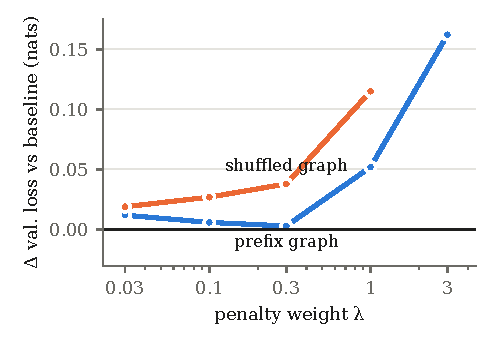
\includegraphics[width=0.52\linewidth]{figs/lambda_sweep.pdf}
\caption{Rayleigh prefix-graph penalty, 100M tokens, one seed: validation loss
relative to baseline as a function of $\lambda$. The shuffled control's cost grows
with $\lambda$; the real graph's shrinks until $\lambda=0.3$.}
\label{fig:lambda}
\end{figure}

\begin{table}[t]
\centering
\small
\begin{tabular}{lcccc}
\toprule
condition ($\lambda=0.3$, Rayleigh) & $\Delta$ val.\ loss & seed std & ratio (prefix) & ratio (substring) \\
\midrule
baseline (4.0042)          & ---      & 0.0021 & 0.80 & 0.84 \\
substring poset            & +0.0015  & 0.0018 & 0.25 & 0.25 \\
substring poset, shuffled  & +0.0193  & 0.0065 & 0.85 & 0.88 \\
prefix graph               & +0.0046  & 0.0002 & 0.19 & 0.33 \\
prefix graph, shuffled     & +0.0253  & 0.0012 & 0.89 & 0.91 \\
\bottomrule
\end{tabular}
\caption{In-domain effect of the Rayleigh penalty (51M model, 250M tokens, 2
seeds).}
\label{tab:rayleigh}
\end{table}

% =============================================================================
\section{A loophole, and the fix}\label{sec:loophole}

\paragraph{Out-of-domain damage.} We evaluate every checkpoint on 2M-token sets of
Python code, arXiv and PubMed articles, and Italian, German and Russian Wikipedia,
where tokens rare in FineWeb-Edu are common. The Rayleigh penalties cost
$+0.11$ to $+0.25$ nats on code, arXiv and PubMed---10--60$\times$ the seed noise---while
their shuffled controls stay near zero. A per-token-type breakdown attributes the
damage to about eight brace tokens (\tok{\{}, \tok{\vsp\{}, \tok{\}}, \tok{\vsp\}},
\tok{\{\textbackslash}, \tok{\}\}}, \tok{\},}, \tok{\})}), each 15--50 nats worse per
occurrence. They occur 0--218 times in the training data.

\paragraph{Mechanism.} Their embedding norms explain it (Table~\ref{tab:norms}).
$R(E)$ is scale-invariant as a whole but not per row. Let $S$ be a set of rows the
language-model loss barely touches (tokens absent from training) that are mutually
smooth on the graph. Scaling them by $c$ gives
\begin{equation}
  R(c) \;=\; \frac{A + c\,B + c^2 B_S}{D + c^2 N_S}
  \;\xrightarrow{c\to\infty}\; \frac{B_S}{N_S},
\end{equation}
where $B_S$ and $N_S$ are the Dirichlet energy and squared norm of $S$ alone. If $S$
is smoother than the embedding as a whole ($B_S/N_S<R$), growing it lowers the
penalty for free. Clusters of unseen, mutually linked tokens (braces, \tok{\textbackslash r},
\tok{\textbackslash t}) are exactly such sets, and under the real graphs they grew about
15$\times$. The shuffled graph links them to random, mostly trained tokens, forms no
such cluster, and nothing inflates. An unseen token adjacent to a well-trained one
(\tok{\textbackslash n\textbackslash n} next to \tok{\textbackslash n}) is instead pulled
toward it and improves by 5 nats per occurrence on code.

\begin{table}[t]
\centering
\small
\begin{tabular}{lcccc}
\toprule
token & baseline & prefix (Rayleigh) & substring (Rayleigh) & prefix, shuffled \\
\midrule
\tok{\{}                        & 1.39 & 21.4 & 21.1 & 0.94 \\
\tok{\vsp\{}                     & 1.39 & 21.6 & 20.8 & 2.77 \\
\tok{\}}                        & 0.89 & 16.0 & 14.8 & 0.65 \\
\tok{\textbackslash r}          & 1.40 & 13.1 & 13.8 & 2.00 \\
\tok{\textbackslash n\textbackslash n} & 1.39 & 0.54 & 0.57 & 0.63 \\
median over all tokens          & 0.91 & 0.83 & 0.82 & 0.91 \\
\bottomrule
\end{tabular}
\caption{Embedding row norms after training. Under the real-graph Rayleigh penalty,
clusters of tokens unseen in training inflate; trained tokens do not.}
\label{tab:norms}
\end{table}

\paragraph{A fix that does not work.} Dropping every edge that touches a token seen
fewer than $N$ times leaves the loophole open for rare-but-seen tokens: with
$N=1$, \tok{\}} (seen 218 times) still inflates and costs 21--28 nats per occurrence,
and the variant is $+0.07$ to $+0.08$ worse than baseline on code, arXiv and PubMed.
(A first implementation also left the masked rows in the denominator, which let
\emph{every} excluded row grow for free; we report it only because it is an easy
mistake to make.)

\paragraph{The fix: a cosine penalty.} Applying the same Laplacian energy to
unit-normalised rows,
\begin{equation}
  P_{\cos}(E) \;=\; \sum_{i<j} a_{ij}\,
  \Big\lVert \frac{e_i}{\lVert e_i\rVert}-\frac{e_j}{\lVert e_j\rVert}\Big\rVert^2,
  \qquad a_{ij}=\frac{w_{ij}/\sqrt{d_i d_j}}{\sum_{k<l} w_{kl}/\sqrt{d_k d_l}},
\end{equation}
makes the penalty invisible to row norms: its gradient with respect to $e_i$ is
orthogonal to $e_i$, so there is nothing to gain by growing. Under it the brace
norms stay at 1.8 (baseline 1.4).

% =============================================================================
\section{Results with the cosine penalty}\label{sec:cosine}

Figure~\ref{fig:ood} summarises the cosine prefix-graph penalty at $\lambda=0.1$ in
three settings; Table~\ref{tab:cosine} gives the 4-seed numbers for the main setting
together with $\lambda=0.03$.

\begin{figure}[t]
\centering
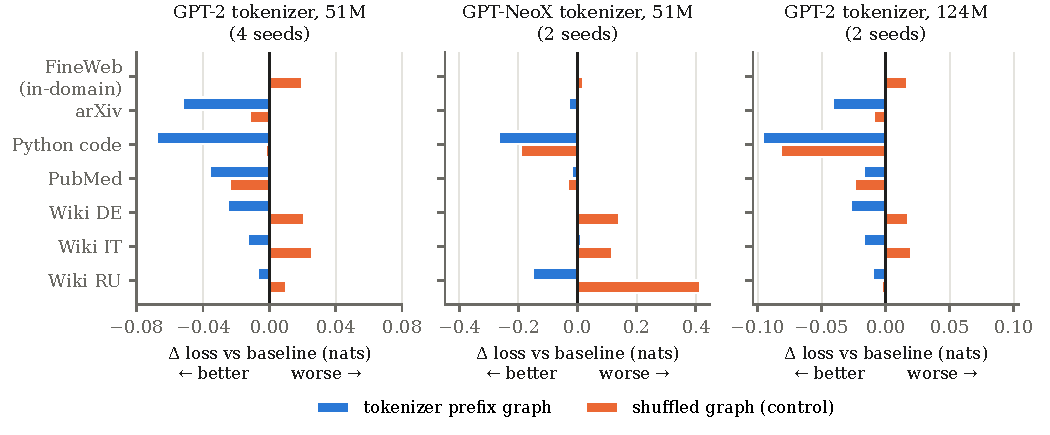
\includegraphics[width=\linewidth]{figs/ood_cosine.pdf}
\caption{Cosine prefix-graph penalty ($\lambda=0.1$), change in mean loss relative
to each setting's own baseline, on the in-domain FineWeb validation set and six
out-of-domain sets. Blue: tokenizer prefix graph. Orange: the same penalty on a
vertex-relabelled graph. Note the different horizontal scales: the GPT-NeoX
tokenizer encodes Cyrillic and code whitespace with tokens that are rare in
FineWeb, which enlarges both the gains and the control's damage.}
\label{fig:ood}
\end{figure}

\begin{table}[t]
\centering
\small
\begin{tabular}{lccccc}
\toprule
evaluation set & \multicolumn{2}{c}{$\lambda=0.1$ (4 seeds)} & \multicolumn{2}{c}{$\lambda=0.03$ (2 seeds)} & baseline \\
\cmidrule(lr){2-3}\cmidrule(lr){4-5}
 & prefix & shuffled & prefix & shuffled & seed std \\
\midrule
FineWeb (in-domain) & \better{$-0.0002$} & $+0.020$ & $+0.001$ & $+0.012$ & 0.0096 \\
arXiv               & \better{$-0.052$}  & $-0.012$ & $-0.047$ & $-0.025$ & 0.0035 \\
Python code         & \better{$-0.068$}  & $-0.002$ & $-0.067$ & $-0.024$ & 0.023 \\
PubMed              & \better{$-0.036$}  & $-0.024$ & $-0.025$ & $-0.050$ & 0.010 \\
Wikipedia DE        & \better{$-0.025$}  & $+0.021$ & $-0.032$ & $-0.009$ & 0.025 \\
Wikipedia IT        & \better{$-0.013$}  & $+0.026$ & $+0.000$ & $+0.018$ & 0.023 \\
Wikipedia RU        & \better{$-0.007$}  & $+0.010$ & $-0.001$ & $-0.002$ & 0.013 \\
\bottomrule
\end{tabular}
\caption{Cosine prefix-graph penalty, 51M model, GPT-2 tokenizer, 250M tokens:
change in mean loss (nats) relative to the 4-seed baseline. FineWeb uses 5M
validation tokens, the other sets 2M.}
\label{tab:cosine}
\end{table}

\paragraph{Free in-domain, better out of domain.} At $\lambda=0.1$ the penalty is
free in-domain (3.9982 vs 3.9983 over 4 seeds) while the embedding stays smoothed on
the prefix graph (ratio 0.49 vs 0.80). Paired by seed, it beats the baseline in 23
of 24 out-of-domain comparisons (the exception: one Russian seed, by $+0.005$) and
beats its shuffled control in 23 of 24. The gain concentrates on tokens rare or
absent in training (\tok{\textbackslash n\textbackslash n}, braces, \tok{\^{}\{},
\tok{\_\{}), which improve by 3--7 nats per occurrence as they inherit from trained
prefix relatives.

\paragraph{Generic versus structural.} At $\lambda=0.03$ the shuffled control also
improves code, arXiv and especially PubMed: any mild smoothing keeps unseen tokens
from drifting to extreme logits. The tokenizer graph adds a margin on top, clearest at
$\lambda=0.1$, where the shuffled penalty already costs $+0.020$ in-domain and the
real one costs nothing. PubMed is the one set where the control is consistently as
good or better---generic smoothing of unseen \LaTeX{} tokens is all that helps there.

\paragraph{Another tokenizer.} With the GPT-NeoX tokenizer (Pythia's), re-tokenizing
both training data and evaluation sets, the penalty is again free in-domain
($-0.0001$; shuffled $+0.021$, 2 seeds). The real-vs-shuffled gap is the largest we
observe: $-0.57$ on Russian, $-0.14$ on German, $-0.10$ on Italian. NeoX encodes
Cyrillic with multi-byte tokens that are rare in FineWeb (81\% of Russian targets);
tied to their real prefix relatives they improve ($-0.153$), tied to random tokens
they get much worse ($+0.416$).

\paragraph{A larger model.} At 124M parameters (GPT-2 small, context 1024, 500M
tokens, 2 seeds) the penalty is free in-domain ($+0.0009$; shuffled $+0.017$ in both
seeds), beats the baseline on all six out-of-domain sets and its shuffled control on
five (PubMed again the exception). A single-seed $+0.01$ in-domain cost seen first
disappeared with the second seed. $\lambda=0.03$ (one seed) is also free, with equal
or larger out-of-domain gains, more of them generic.

% =============================================================================
\section{Discussion}

\paragraph{What the tokenizer knows.} Embeddings learned without any constraint
already respect the tokenizer's word-boundary structure (Section~\ref{sec:pretrained}),
and forcing more of it costs nothing in-domain. The useful information is not in
frequent tokens---the model learns those from data---but in the long tail: a token
the corpus rarely or never shows still has a string, and its prefix relatives are a
far better guess for its embedding than its random initialisation. The cosine
penalty turns that into a training signal. Relabelled graphs do not provide it, which
is why they cost in-domain and help out of domain only through generic smoothing.

\paragraph{The penalty's form matters.} The obvious scale-invariant regulariser is
not safe: any rows the loss ignores can game a global normalisation. Row
normalisation removes the degree of freedom. The general lesson for structural priors
on embeddings is to check what happens to rows the data does not constrain.

\paragraph{Limitations.}
\begin{itemize}
  \item \emph{Scale.} The largest model is 124M parameters trained on 500M tokens;
  seeds are 4 (51M), 2 (NeoX, 124M) and 1 (some $\lambda$ variants). Whether the
  in-domain cost stays at zero for much larger models and longer training is open.
  \item \emph{One training corpus.} FineWeb-Edu is filtered English; the
  out-of-domain gains are gains on text that corpus rarely contains. With a
  multilingual or code-heavy corpus the long tail shrinks and so, presumably, does
  the effect.
  \item \emph{Evaluation sets.} The arXiv and PubMed sets are lower-cased with
  spaced punctuation and \texttt{@xmath} placeholders; per-bucket averages over rare
  tokens can be dominated by a few token types, so we rely on all-token means.
  \item \emph{Tokenizers.} Two 50k byte-level BPE vocabularies; 128k vocabularies
  (Llama~3) were only analysed, not trained with.
\end{itemize}

% =============================================================================
\section{Conclusion}

A tokenizer's vocabulary is a structured object, and pretrained embeddings reflect
its word-boundary structure in a nearly scale-invariant way. Imposing that
structure through a row-normalised Laplacian penalty on the prefix graph is free on
in-domain text and improves out-of-domain loss by letting rare and unseen tokens
inherit from their prefix relatives. The effect survives four seeds, a second
tokenizer and a 2.4$\times$ larger model, and is clearly separated from generic
regularisation by a relabelled-graph control. The most natural next steps are larger
models and corpora, and weighting the penalty by token frequency so that it acts
where data is scarce.

% =============================================================================
\appendix
\section{Reproducibility}

All code, tests and the Colab notebook are in the \texttt{Tokenix} repository.
\begin{itemize}
  \item \texttt{experiments/pretrained\_probe.py}: Section~\ref{sec:pretrained}
  (GPT-2, Pythia, Llama-3.2-1B; only embedding tensors are downloaded).
  \item \texttt{experiments/prepare\_data.py}, \texttt{prepare\_eval\_sets.py}:
  FineWeb-Edu and the six out-of-domain sets; the tokenizer is recorded in each data
  folder's \texttt{meta.json}.
  \item \texttt{experiments/train\_gpt.py}: training. Flags:
  \texttt{--condition} (\texttt{baseline}, \texttt{prefix}, \texttt{contain},
  optionally suffixed \texttt{:shuffled}), \texttt{--penalty} (\texttt{rayleigh} or
  \texttt{cosine}) and \texttt{--lam}. The penalty itself is in
  \texttt{tokenix/torch\_penalty.py}.
  \item \texttt{experiments/eval\_by\_frequency.py}, \texttt{token\_diagnostics.py}:
  loss by token frequency and by token type.
  \item \texttt{notebooks/colab\_train.ipynb}: every run reported here (steps 3--15).
  \item \texttt{paper/make\_figures.py}: the figures in this document.
\end{itemize}

\begin{table}[h]
\centering
\small
\begin{tabular}{lcc}
\toprule
 & 51M & 124M \\
\midrule
layers / width / heads / context & 8 / 512 / 8 / 512 & 12 / 768 / 12 / 1024 \\
tokens per step & 131{,}072 & 262{,}144 \\
training tokens & 250M & 500M \\
peak lr / warmup / min lr & $10^{-3}$ / 500 / 10\% & $6\cdot10^{-4}$ / 500 / 10\% \\
optimiser & \multicolumn{2}{c}{AdamW, $\beta=(0.9,0.95)$, weight decay 0.1, grad clip 1.0} \\
precision & \multicolumn{2}{c}{bf16 autocast, \texttt{torch.compile}, one A100} \\
\bottomrule
\end{tabular}
\caption{Training hyperparameters.}
\end{table}

% =============================================================================
\begin{thebibliography}{9}\small
\bibitem{chung1997} F.~R.~K. Chung. \emph{Spectral Graph Theory}. CBMS Regional
Conference Series in Mathematics 92, American Mathematical Society, 1997.
\bibitem{sennrich2016} R.~Sennrich, B.~Haddow, A.~Birch. Neural machine translation
of rare words with subword units. \emph{ACL}, 2016.
\bibitem{radford2019} A.~Radford, J.~Wu, R.~Child, D.~Luan, D.~Amodei,
I.~Sutskever. Language models are unsupervised multitask learners. OpenAI, 2019.
\bibitem{ethayarajh2019} K.~Ethayarajh. How contextual are contextualized word
representations? Comparing the geometry of BERT, ELMo, and GPT-2 embeddings.
\emph{EMNLP}, 2019.
\bibitem{gao2019} J.~Gao, D.~He, X.~Tan, T.~Qin, L.~Wang, T.-Y.~Liu. Representation
degeneration problem in training natural language generation models. \emph{ICLR},
2019.
\bibitem{land2024} S.~Land, M.~Bartolo. Fishing for Magikarp: automatically detecting
under-trained tokens in large language models. \emph{EMNLP}, 2024.
\bibitem{penedo2024} G.~Penedo et al. The FineWeb datasets: decanting the web for the
finest text data at scale. \emph{NeurIPS Datasets and Benchmarks}, 2024.
\end{thebibliography}

\end{document}
